In order to evaluate our proposal, we ran experiments over two standard corpora, namely: 20 Newsgroup\footnote{http://qwone.com/\~jason/20Newsgroups} and Reuters50\footnote{https://archive.ics.uci.edu/ml/datasets/Reuter\_50\_50}. The first one consists of 13000 messages taken from 20 newsgroups, whereas the second one contains 5000 documents authored by 50 different authors. Table~\ref{} summarizes the characteristics of the two corpora. Each corpus is divided in a training and test set with a ratio 80-20 percent. Models are evaluated according to their perplexity on the test set and we follow here the  approach of \cite{asuncion_smoothing_2009} based on the following fold-in procedure: the word-topic distribution is learned on the training set and considered fixed, whereas the document-topic distribution is learned for each document of the test set, by using the first half of the document only; the perplexity is then computed on each test document, then averaged over all test documents, using:
%
\[
\begin{array}{l@{\hspace{.3cm}}l}
\log p(x^{test}) = \sum_{dw} n_{dw} \log \sum_k \hat{\theta}_{kd} \hat{\phi}_{wk} \\
perplexity(x^{test}) = \exp(- \frac{\log p(x^{test})}{\sum_d n_d})
\end{array}
\]
%
with $n_d = \sum_w n_{dw}$.

We have compared several variants of the LDA model according to the previous development:
%
\begin{itemize}
\item With a symmetric prior, fixed or estimated with the EM type 2 procedure, for $\alpha$ and/or $\beta$;
\item With a fixed asymmetric prior, for $\alpha$ and/or $\beta$;
\item With a Boojum prior, estimated with the procedure described in Section~\ref{sec:LDAwithPrior}, for $\alpha$ and/or $\beta$.
\end{itemize}
%
The best combination is obtained with a fixed asymmetric prior on $\alpha$ and a Boojum on $\beta$. In the remainder, we refer to this model as {\it conjugate LDA} ({\it ldaconjugate} for short). Both the Boojum prior and the asymmetric prior on $\alpha$ yield better results than the symmetric one, in acordance with the results obtained in \cite{wallach_rethinking_2009} which illustrate the imporatnce of an asymmetric prior on the document-topic distribution. Furthermore, the Boojum prior on $\beta$ helps here to improve the models.

Figure~\ref{fig:pp-exple} illustrates the behavior of the conjugate LDA model wrt to the standard LDA model (with symmetric priors estimated via the EM type 2 procedure). The perplexity is averaged over 10 runs to assess the influence of the random initilization of the parameters. The number of topics is set to 6 and the number of documents to 1000. As one can note, the perplexity of the conjugate model is lower than the one of the standard model, and decreases with the number of iterations, as expected. The Boojum prior on the word-topic distribution leads to a higher decrease in perplexity.

\begin{figure}[h]
\label{fig:pp-exple}
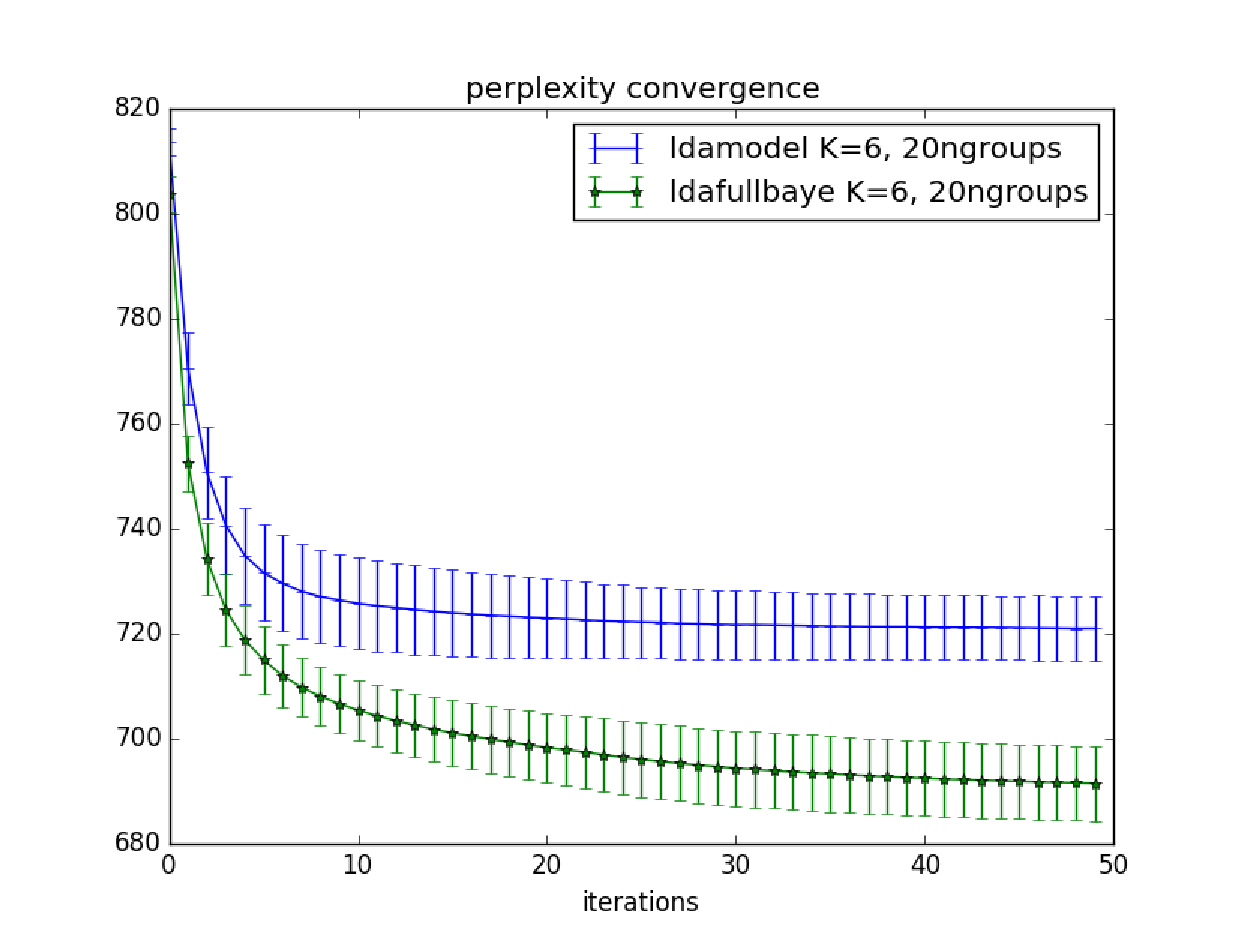
\includegraphics[scale=0.4]{results/pp_conv}
\caption{Evolution of perplexity on the test sets according to the number of iterations of the variationnal Bayes methods for both conjugate and standard LDA mdoels, for 20 Newsgroup}
\end{figure}


Figure~\ref{fig:pp-size} shows how the conjugate LDA model behaves, compared to the standard LDA model, with respect to the size of the collection. Here again, the number of topics $K$ is first set to $6$ and the curves correspond to the ratio of perplexity of the conjudate LDA model wrt to the standard LDA model. As one can note, the ratio of perplexity is below $1$ when the size of the collections is small (roughly below 3000 documents), and above 1 after that. This indicates that the conjugate LDA model compares favorably to the standard model for small collections, which can be explained by the additional information brought by the prior on such collections (the influence of the prior then decreases with the size of the collection). Figure~\ref{fig:pp_D} also displays the ratio of perplexity for the two collections with the number of topics set to the actual number of classes in the collections: $K=20$ for 20 Newsgroup, as the data originates from $20$ different news groups, and $K=50$ for Reuters50 as the texts are authored by $50$ different persons. As one can note, we observe the same tendency as the one mentioned above, even though the difference between the two models is less marked.

\begin{figure}[ht]
\label{fig:pp-size}
%\vspace{.3in}
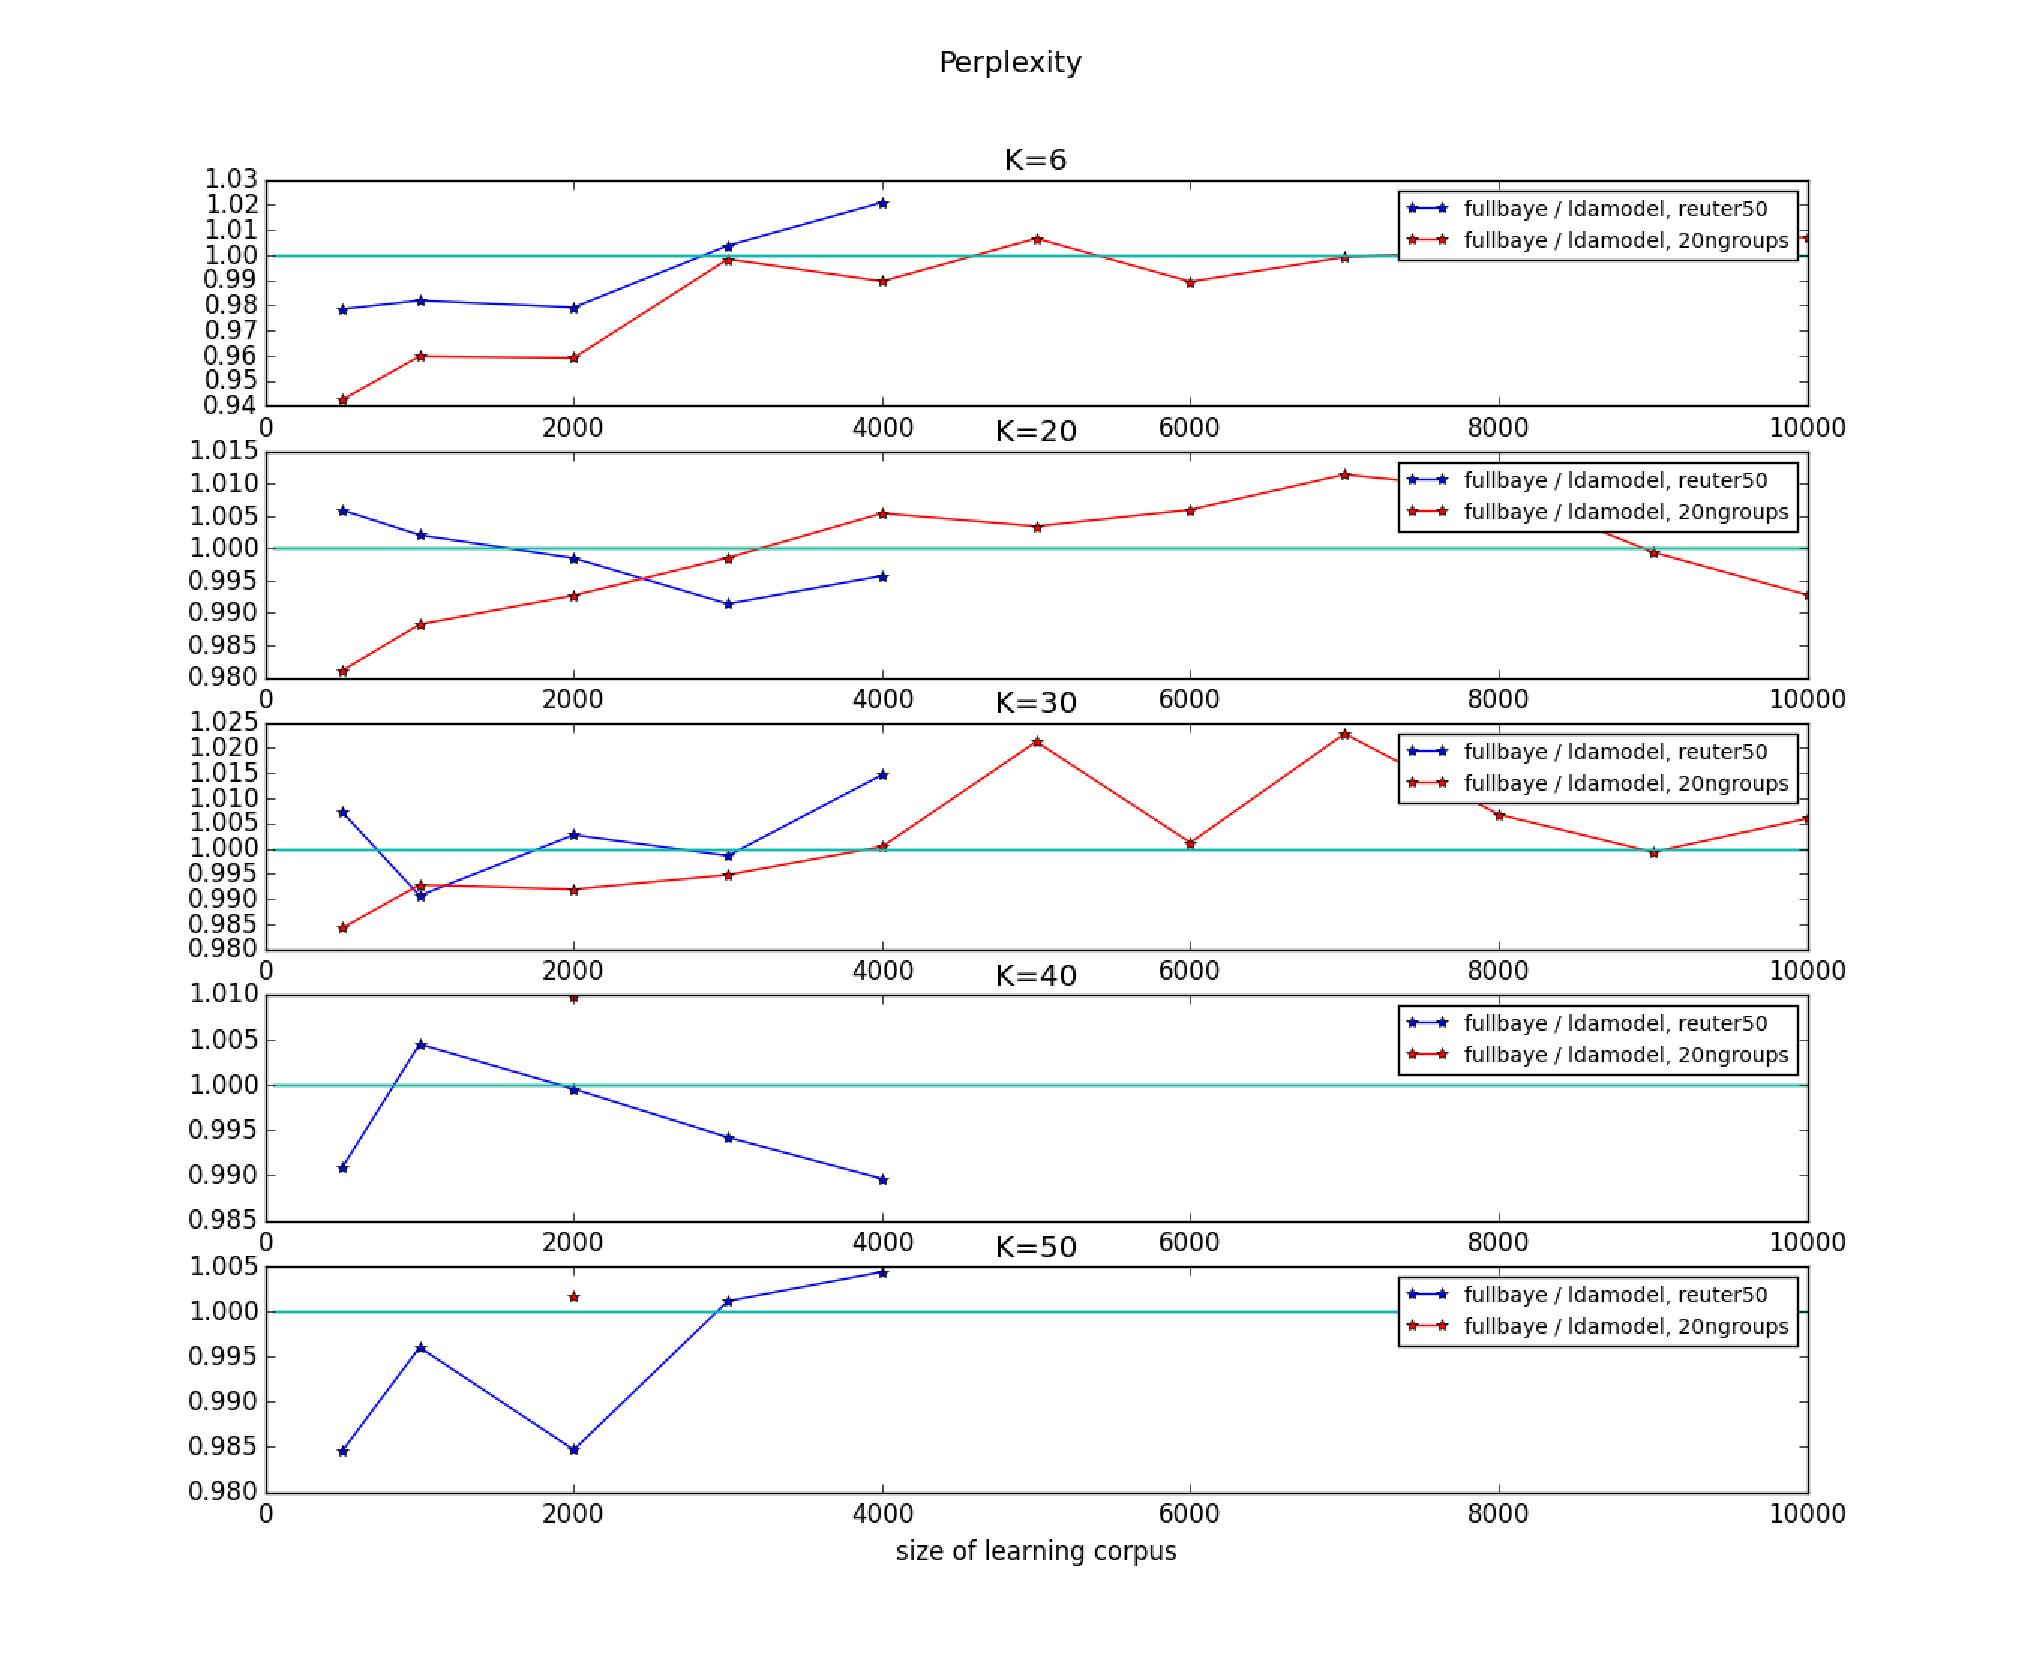
\includegraphics[width=9cm, height=14cm]{results/pp_D}
%\vspace{.3in}
\caption{Perplexity ratio for the conjugate LDA model and the standard LDA model according to the size of the collection ($K=6,20$ for 20 Newsgroup and $K=6,50$ for Reuters50)}
\end{figure}


\textcolor{red}{To be kept and completed if we have a nice illustration!\\ Figure~\ref{fig:3} illustrates the qualitative impact of the Boojum prior on the word-topic distribution.}

Lastly, Figure~\ref{fig:time} compares the execution time of the inference procedures for the two models for $K=20$. Similar plots are obtained for different values of $K$. As one can note, there is no significant difference between the inference in the conjugate and the standard models.

\begin{figure}[h]
\label{fig:time}
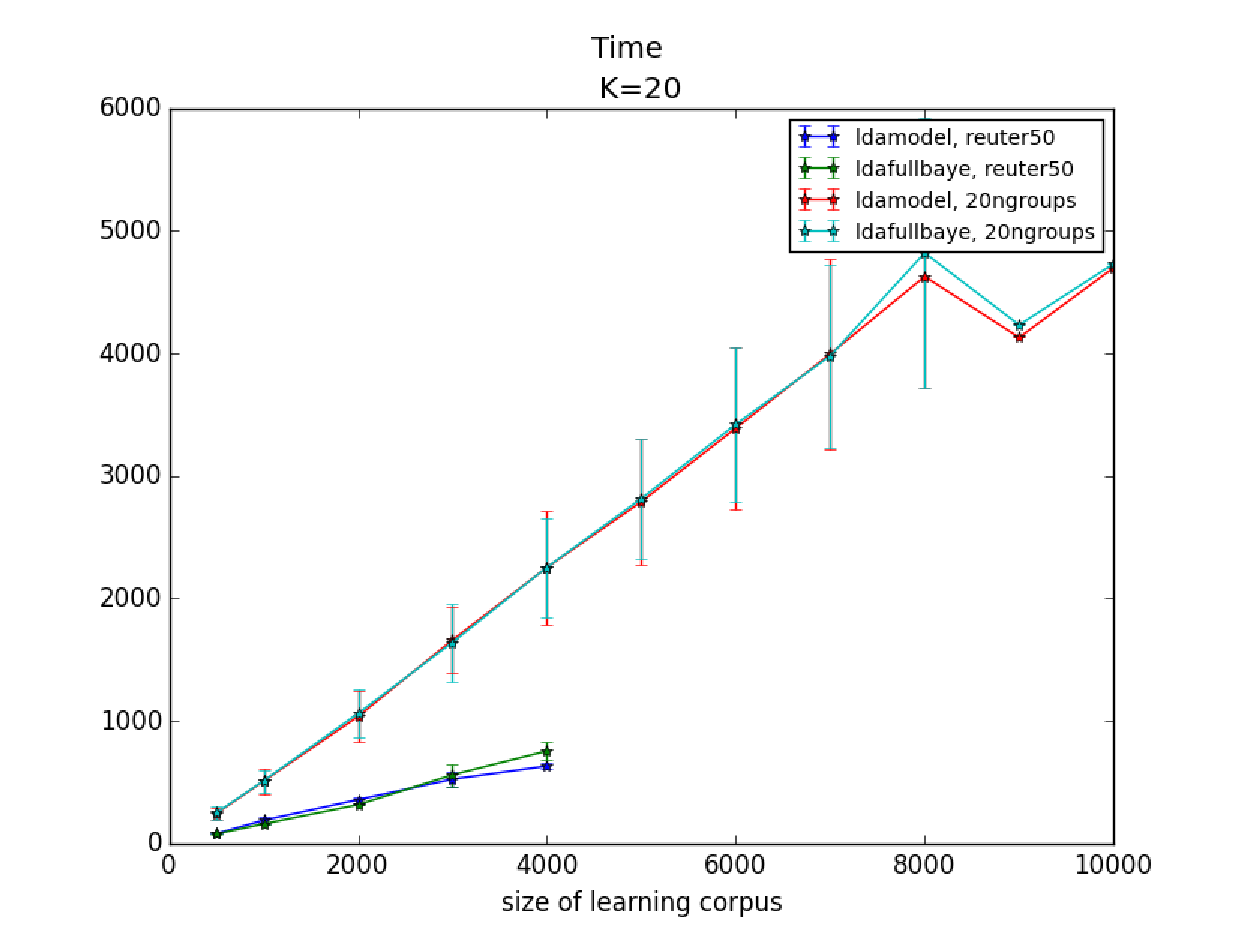
\includegraphics[scale=0.4]{results/time}
\caption{Time of inference for 50 iterations of variational bayes.}
\end{figure}
